We conducted several numerical experiments to confirm the validity of the error bounds formed in \cref{sec:mpanalysis}.
First, we tested \cref{algo:hhQR,algo:blockHQR,algo:par_tsqr,algo:mpBQR}, {\tt mpHQR2}, {\tt mpBQR2}, and {\tt mpTSQR2} for varying matrix sizes.
Then, we tested varying block sizes in \cref{algo:mpBQR} for a fixed matrix size, and lastly compared the performance of {\tt mpHQR2} and {\tt mpTSQR2}.\par

In \cref{sec:mpanalysis}, we gave the forward error bounds for $\bb{R}$ and $\bb{Q}$ separately. 
Since our numerical experiments measure $\|\hat{\bb{Q}}\hat{\bb{R}}-\bb{A}\|_F$ and $\|\hat{\bb{Q}}^{\top}\hat{\bb{Q}}-\bb{I}\|_2$ instead, we show how to convert the forward errors in general.
Given $\|(\hat{\bb{R}}-\bb{R})[:,j]\|_2\leq \epsilon_R \|\bb{A}[:,j]\|_2$ and $\|(\hat{\bb{Q}}-\bb{Q})\|_F\leq \epsilon_Q$,
\begin{align}
	\|(\hat{\bb{Q}}\hat{\bb{R}}-\bb{A})[:,j]\|_2 &\leq (\epsilon_R+\epsilon_Q + \epsilon_R\epsilon_Q)\|\bb{A}[:,j]\|_2,\;\; j=1:n,\quad \text{see \cite{Higham2002}},\\
	\|\hat{\bb{Q}}\hat{\bb{R}}-\bb{A}\|_F &\leq n^{1/2}(\epsilon_R+\epsilon_Q + \epsilon_R\epsilon_Q)\|\bb{A}\|_F, \label{eqn:QRA} \\
	\|\hat{\bb{Q}}^{\top}\hat{\bb{Q}}-\bb{I}\|_2 &\leq \|\hat{\bb{Q}}^{\top}\hat{\bb{Q}}-\bb{I}\|_F \simeq 2\epsilon_Q,\quad\text{see \cite{Mori2012}} \label{eqn:QQI}.
\end{align}
%\subsection{Varying matrix sizes}
%\subsection{Varying block sizes in {\tt mpBQR3}}

\begin{figure}[h!]%{r}{.53\textwidth}
	\centering
	\vspace{-10pt}
	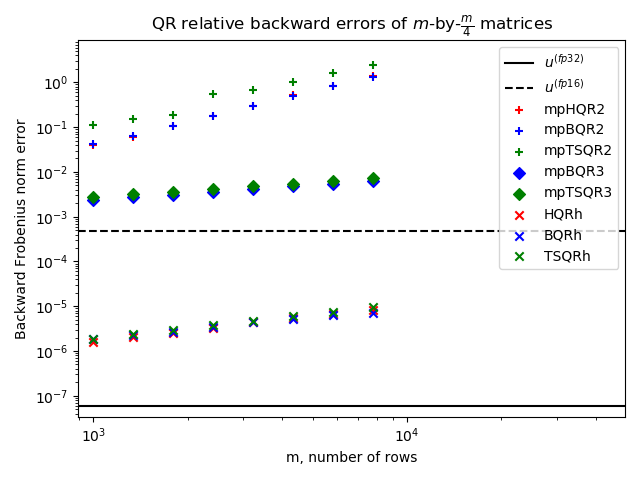
\includegraphics[width=0.45\textwidth]{./figures/sizefig.png}
	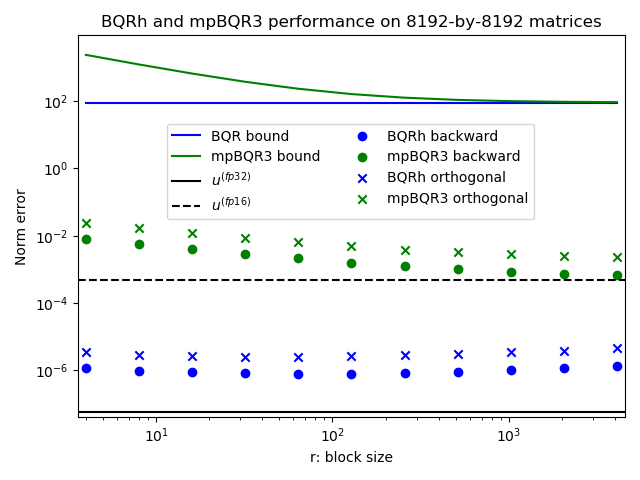
\includegraphics[width=0.45\textwidth]{./figures/mpBQR3-blocksize.png}
	\caption{\label{fig:sizempBQR3}Left plot: Relative backward error of all HH QR factorization algorithms discussed in \cref{sec:algo,sec:mpanalysis} with varying matrix sizes. Right plot: Relative backward error of {\tt mpBQR3} for $8192$-by-$8192$ matrices are shown with block size $r$ ranging from $4$ to $4096$.}
	\vspace{-10pt}
\end{figure} 
%\subsection{Varying condition numbers}
Lastly, we compared HQR and TSQR performances in the mixed precision setting described in \cref{assump:mp}.
Note that an empirical comparison of the two algorithms were reported in \cite{Mori2012} in fp64 arithmetic, and we omit the comparison against {\tt mpBQR2} since it performs very similarly to {\tt mpHQR2}.
%TODO: talk why omit BQR? or wait for BQR
The numerical experiments show that TSQR can outperform HQR in mixed precision settings in practice even though the theoretical bounds do not guarantee stability.
In addition, the empirical results do not always behave in the same trend as the theoretical bounds suggest, which highlights the shortcomings of deterministic error bounds that are too pessimistic. \par
We used Julia, which allows fp16 storage and {\tt castup} and {\tt castdown} operations between types in {fp16, fp32, fp64}, but no built-in fp16 arithmetic.
Therefore, we relied on using Algorithm~\ref{algo:simulate} for $f\in \text{OP} \cup\{{\tt dot\_product}\}$ to simulate \cref{assump:mp}.
Following example from \cite{Mori2012}, we used $m$-by-$n$ random matrices, $\bb{A}_{\alpha}$, constructed via
\begin{equation}
\bb{A}_{\alpha} = \bb{Q'}(\alpha \bb{E} + \bb{I})/\|\bb{Q'}(\alpha \bb{E} + \bb{I})\|_F,
\label{eqn:genRM}
\end{equation}
where $\bb{Q'}\in\mathbb{R}^{m\times n}$ is a random orthogonal matrix and $\bb{E}\in\R^{n\times n}$ is the matrix of $1$'s. 
We constructed $\bb{Q'}$ by computing the default QR factorization of matrix $\bb{\Omega}\in\F_{fp64}^{4000\times100}$ in Julia, which performs BQR with $r=36$ entirely in fp64 arithmetic.                                                                                                                    ents of the random matrix $\bb{\Omega}$ were sampled from $Unif(0,1)\cap \F_{fp64}$.
By construction, $\bb{A}_{\alpha}$ has 2-norm condition number $n\alpha+1$. 
By varying $\alpha$ from {\tt 1e-4} to {\tt 1}, we varied the condition number from $1.1$ to $101$, and we generated $10$ samples for each value of $\alpha$.
The relative backward error, $\|\hat{\bb{Q}}\hat{\bb{R}}-\bb{A}\|_F/\|\bb{A}\|_F$, was computed by casting up $\hat{\bb{Q}}$, $\hat{\bb{R}}$, and $\bb{A}$ to fp64 to compute the Frobenius norms.
Note that plugging in $m=4000$, $n=100$, $u^{(l)}=u^{(fp16)}$, $u^{(h)}=u^{(fp32)}$, and $c=1$ (for $\tilde{\gamma}$) into the error bounds for {\tt mpHQR2} combined with \cref{eqn:QRA,eqn:QQI} are approximately {\tt 1.179} and {\tt 1.146}.
These error bounds are \emph{relative} and these worst-case bounds do not guarantee errors below 100\%.
The TSQR bounds for the same parameters for $L=1:5$ are even larger, which indicates that stability is not guaranteed. 
\begin{wrapfigure}{l}{.4\textwidth}
	\centering
	\vspace{-10pt}
	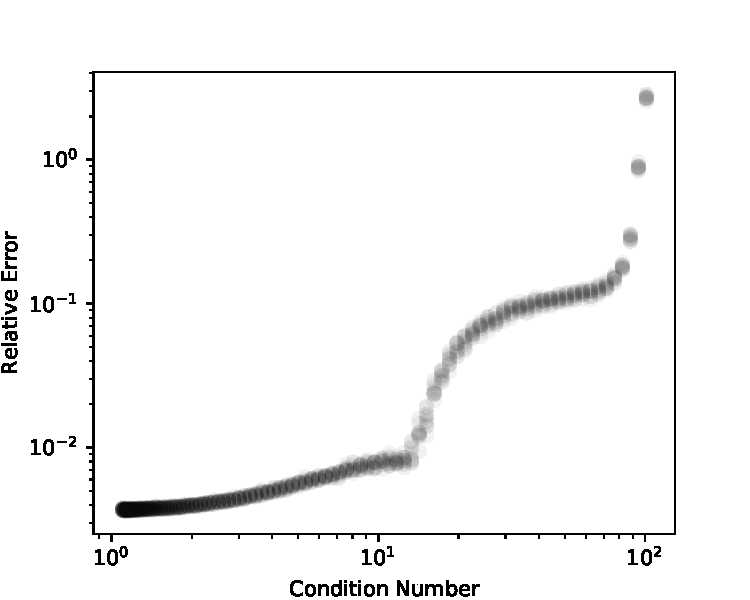
\includegraphics[width=.3\textwidth]{./figures/unblocked.pdf}
	\caption{\label{fig:unblocked} HQR errors for matrices with varying condition numbers.}
	%\vspace{-10pt}	
\end{wrapfigure}
Figure~\ref{fig:unblocked} shows the backward errors of {\tt mpHQR2} increasing as the theoretical condition numbers of the generated random matrices increase, and these errors correspond to the error data on the vertical axis, $L=0$, of Figure~\ref{fig:allTSQR}.
In addition to the errors from {\tt mpHQR2}, Figure~\ref{fig:allTSQR} shows the errors from {\tt mpTSQR2s} of levels varying from $L=1$ to $L=5$, where each line represents the errors of HQR and variants of TSQR calculated from the same random test matrix.
Figure~\ref{fig:allTSQR} reveals two different trends for the errors as we deepen the complexity of the QR algorithm from {\tt mpHQR2} to {\tt mpTSQR2} with $L=5$. 
One trend occurs for matrices with smaller condition numbers, where {\tt mpHQR2} is stable, but {\tt mpTSQR2} with higher levels yield larger errors. 
Another trend occurs for matrices with higher condition numbers, where single-level and 2-level {\tt mpTSQR2} yield smaller errors than {\tt mpHQR2}. 
In these cases, errors from {\tt mpTSQR2} with 3 or more levels are similar to or worse than their 2-level variants, but generally do not exceed those of {\tt mpHQR2} most of the times.
These results suggests that TSQR can outperform HQR even in mixed precision settings, and particularly when HQR is unstable due to larger condition numbers.
Although this experiment focused on condition numbers, identifying other properties that point to better performance of TSQR than HQR can further broaden the potential use of mixed precision TSQR in applications.
%The first trend When the error is low enough for the unblocked QR factorization, TSQR performs worse for these matrices.
%Recall that machine precision for half-precision is about $10^{-3}$. 
%This shows that the traditional QR factorization had been very good to begin with.
%Finally, even when TSQR is \textit{successful} initially, we can see that too many initial blocks can become a problem as well. 
%
%Overall, this figure shows a variety of results that encourage further exploration. 
%We have shown that TSQR can improve on certain matrices where the unblocked HQR algorithm was highly unstable in half-precision.
%Identifying which matrix properties correlate to TSQR and why can help broaden the possibility of using lower precision arithmetic for QR factorizations.

\begin{figure}[h!]%{r}{.53\textwidth}
	\centering
	%\vspace{-10pt}
	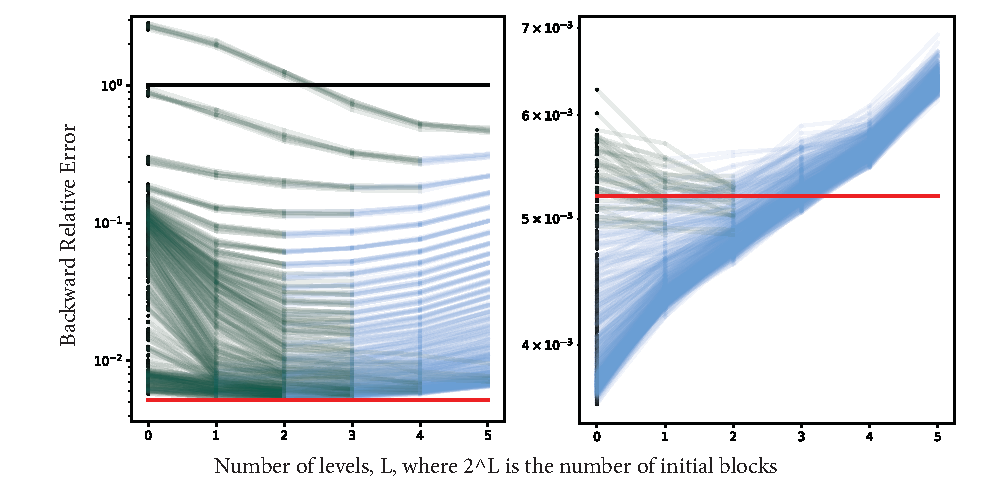
\includegraphics[width=0.8\textwidth]{./figures/allTSQR2.pdf}
	\caption{\label{fig:allTSQR} Left plot shows the relative error of QR factorization for matrices with condition numbers ranging from 5.3 to 101, and the right plot shows the errors for matrices with condition numbers ranging from 1.1 to 5.3. }
	\vspace{-10pt}
\end{figure} 
